\chapter{Funktionsweise}\label{ch:operatingPrinciple}

Beim Reed-Solomon Verfahren werden die zu codierenden Nachrichten in Symbole $m_{i}$ der Länge 8 Bit zusammengefasst.
Die zu übermittelnden oder zu speichernden Daten werden also nicht dirket als Bitstrom verarbeitet, obwohl sie als Bits vorliegen.
Eine binäre Nachricht wird in 8 Bit-lange Teile aufgesplittet und dann jeweils als ein Symbol interpretiert.
Die Anzahl dieser Symbole ist dann die Nachrichtenlänge $k$.
Ein Nachricht $m$ hat also die Form $[m_{0}m_{1}m_{2}...m_{k-1}]$.

Zum Beispiel wird eine Nachricht mit dem Bitmuster $0010100110100101$ in $00101001\ 10100101$ zerlegt und einzeln in Symbole übersetzt (hier Decimaldarstellung) $41\ 165$. Hier wäre die Nachrichtenlänge 2.

Nach Hinzufügen der Redundanzsymbole durch Encodieren entsteht ein Block der Länge $n$.
Die Spezifikation der Ausprägung des eingesetzen Reed-Solomon-Codes wird typischerweiese als $RS(n, k)$ dargestellt.
Die Berechnungen erfolgen dabei in dem endlichen Körper $GF(q)$, wobei $q\geq n>k$ eine Primzahlpotenz ist.

Diese allgemeine Prinzipe gelten für alle Reed-Solomon Varianten. Die folgenden Ausführungen zum Encoding in Abschnitt \ref{sec:encoding} und Decoding in Abschnitt \ref{sec:decoding} beziehen sich auf den ursprünglichen Ansatz von 1960.

\section{Encodierung}\label{sec:encoding}

Die Codierung basiert auf der Multiplikation und Division von Polynomen. 
Aus einer Nachricht  $m=[m_{0}m_{1}m_{2}...m_{k-1}]$ wird das Polynom \[p(x)=\sum_{i=0}^{k-1}m_ix^i=m_0+m_1x+m_2x^2+...+m_{k-1}x^{k-1}\] mit den Nachrichtensymbolen $m_i$ als Koeffizienten der Summanden.
Dieses Polynom wird auch als Nachrichtenpolynom bezeichnet.

Das zu bildendende Codewort $c=[c_{0}c_{1}c_{2}...c_{n-1}]$ hat die Lange $n=k+2t$, also Länge der ursprünglichen Nachricht und die Anzahl der redundanten Symbole. Dadurch können $2t$ Fehler erkannt und $t$ Fehler korrigiert werden.
Das Codewort entsteht durch das Einsetzten von $n$ festen Werten in das Nachrichtenpolynom.
\[c_i=p(q_i)\]
Diese Werte $[q_0 q_1 q_2...q_{n-1}]$ sind die primitiven Elemente des endlichen Körpers über $q$.
Dieses Codewort wird dann gespiechert oder übertragten und kann bis zum Decodieren beschädigt werden.

\section{Decodierung}\label{sec:decoding}

Aus dem Codewort $c=[c_{0}c_{1}c_{2}...c_{n-1}]$ muss zum Decodieren die Nachricht wiederhergestellt werden.
Dazu muss die Encodierung rückgängig gemacht werden, indem für jedes Symbol die Encodierungsgleichung aufgestellt wird mit dem unterschied das nun $p(x)$ unbekannt ist.
\begin{alignat}{5}
	&c_0&&=p(q_0)&&=m_0\nonumber\\
	&c_1&&=p(q_1)&&=m_0+m_1 q_1&&+m_2 (q_1)^2&&+\cdots+m_{k-1} (q_1)^{k-1}\nonumber\\
	&c_2&&=p(q_2)&&=m_0+m_1 q_2&&+m_2 (q_2)^2&&+\cdots+m_{k-1} (q_2)^{k-1}\nonumber\\
	&&&&&&&\cdots\nonumber\\
	&c_{n-1}&&=p(q_{n-1})&&=m_0+m_1 q_{n-1}&&+m_2 (q_{n-1})^2&&+\cdots+m_{k-1} (q_{n-1})^{k-1}\nonumber
\end{alignat}

Dadurch entsteht ein Gleichungssystem mit $n$ Gleichungen und $k$ Unbekannten, den Koeffizienten des Polynoms, welche wiederum die Symbole der Nachricht $m_i$ sind. 
Da $n>k$, reichen $k$ dieser Gleichungen aus, um das Gleichungssystem eindeutig zu lösen und so die Nachricht zu erhalten.

Allerdings funktioniert das so nur in der idealen Welt. 
In der Realität ist das Codewort möglicherweise fehlerbehaftet. 
Einige Symbole von $c$ können also verändert worden sein, sodass ein $\hat{c}$ entsteht. 
Wie viele Fehler und an welchen Stellen diese aufgetreten sind lässt sich nicht a priori nicht sagen. 
So reicht es also nicht aus nur $k$ Gleichungen zum Lösen des Gleichungssystems zu verwenden, da in diesen $k$ Gleichungen ja bis zu $2t$ Fehler enthalten sein können.
Bei mehr als $2t$ Fehlern würde ein falsches Ergebnis das Mehrheitsvoting gewinnen, wodurch die Fehlerkorrektur fehlschlägt.
Trotzdem handelt es sich bei Reed-Solomon um ein Verfahren, das maximal viele Fehler erkennen bzw. korrigieren kann.
Der Hamming-Abstand, eine Kenngröße für die Effektivität von Codierungsverfahren, ist bei Reed-Solomon $n-k+1$, welches den optimalen Trade-Off zwischen Länge der hinzugefügten Redundenz und der Fähigkeit Fehler zu erkennen und zu korrigieren (Singelton-Schranke).
Ein ausführlicher Beweis dazu findent sich in Anhang \ref{app:singeltonBorder}.

Um eine korrekte Lösung des Gleichungssystems zu finden, müssen alle $\binom{n}{k}$ möglichen Gleichungssysteme gelöst werden und dann mit Mehrheitsentscheidung das Ergbebnis mit den meisten Votes ausgewählt werden. 
Wenn man beispielsweise eine typische konfiguration $RS(255,223)$ annimmt, folgen daraus $\binom{255}{223}\approx5\cdot 10^{40}$ Gleichungssysteme, die gelöst werden müssen.
Bei einer Lösungsdauer von einer Millisekunde pro Gleichungssystem, wären das immer noch eine Gesamtdauer von ca. $3,17\cdot10^{29}$ Jahren. 
So kann man leicht nachvollziehen warum dieses Verfahren in dieser Form nicht effizent lösbar ist.

\section{Berlekamp-Welch Algorithmus}\label{sec:bwAlgo}

Der Berlekamp-Welch Algorithmus bietet eine Lösung dieses Problems. 
Definiere ein Fehlerlokator-Polynom $e(x)=(x-e_1)(x-e_2)\cdots(x-e_t)$ mit $deg(e)=t$ und $q(x)=p(x)e(x)$ mit $deg(q)=deg(p)+deg(e)=k-1+t$.
Umgeformt sind die zu besteimmenden Polynome
\begin{alignat}{1}
	&e(x)=1x^t+b_{t-1}x^{t-1}+\cdots+b_1x+b_0\nonumber\\
	&q(x)=a_{k+t-1}x^{k+t-1}+a_{k+t-2}x^{k+t-2}+\cdots+a_1x+a_0,\nonumber
\end{alignat}
welche zusammen $k+2t$ unbekannte Koeffizienten haben.
Die $k+2t$ Symbole des Codeworts liefern also genau genug Informationen um diese Koeffizeinten eindeutik zu besteimmen, indem man $k+2t$ Gleichungen der Form $q(i)=e(i)$ aufstellt, wobei $1\leq i\leq k+2t$.
Mit diesen gegebenen Koeffizeinet sind auch $q(x)$ und $e(x)$ bekannt und es kann durch Polynomdivision wieder das ursprüngliche Polynom $p(x)$ berechnet werden, um damit die Nachricht wie beim Encoding zu bestimmen.

\section{Hardware-Implementierung}\label{sec:hardware}

Um dieses Fehlerkorrektur Verfahren in möglichst vielen Szenarien anwenden zu können, ist es wichtig, dass eine Verwendung fast ohne Beeinträchtigung möglich ist.
Dafür wird häufig auf eine spezielle Implementierung in Hardware gesetzt, um den Einsatz auch auf kleinen Geräten wie Mikrokontrollern zu ermöglichen.
Da viele Algorithmen des Reed-Solomon-Codes auf der Polynomdivision basieren, gibt es dafür dedizierte Hardwarekomponenten.
Eine solche Implementierung zur Polynomdivision, wie in Abbildung \ref{fig:polynomdivCircuit} abgebildet, wird im Folgenden näher beschrieben.
\begin{figure}[ht]
	\centering
	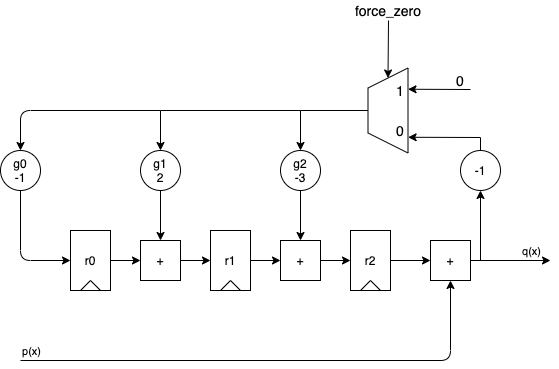
\includegraphics[width=0.9\textwidth]{figures/reed_solomon-divider_diagram.png}
	\caption{Schaltung zur Polynomdivision}
	\label{fig:polynomdivCircuit}
\end{figure}\todo{Grafik überarbeiten}

Die Schaltung arbeitet mit Addierern $a_i$ und Multiplizierern $g_i$ und ist rückgekoppelt, das heißt die Berechnungen basieren auf dem zuvor durchgeführten Berechnungsschritt \cite{masseyShiftregisterSynthesisBCH1969}.
Am Eingang $p(x)$ werden jeweils die Koeffizienten des Dividenden angelegt, am Ausgang $q(x)$ kommen die Koeffizienten des Ergebnissses an, jeweils die Koeffizienten mit dem höchsten Exponenten zu erst.
Der Divisor ist durch die Multiplizierer dargestellt. Bei $g_0$ handelt es sich um den Koeffizenten von $x^0$. 
Dabei werden die Reste eines Divisionsschrites in den Registern $r_i$und sequenziell in den folgenden Iterationen weiterverwendet, wie man es auch mit Stift und Papier durchführen würde.

Mit Hilfe dieser oder ähnlicher Schaltungen und dem in Abschnitt \ref{sec:bwAlgo} genannten Algorithmus war es möglich in den verschiedenten Einsatzbereichen Reed-Solomon zu verwenden.